\chapter{Elasticidades: medir la sensibilidad}
\label{cap:elasticidad}

\section{El problema de las unidades}

Sabemos que si sube el precio, baja la cantidad demandada (Capítulo~\ref{cap:funciones}). Pero, ¿cuánto? La derivada $\dd Q/\dd p$ da una respuesta, con un problema: \textbf{depende de las unidades}. Si mido la cantidad en kilos o en toneladas, o el precio en pesos o en dólares, el número cambia, aunque la realidad económica sea la misma. Para comparar sensibilidades entre productos y mercados necesitamos una medida \emph{sin unidades}. Esa medida es la \textbf{elasticidad}: el cociente de \emph{variaciones porcentuales} \cite{varian}.

\section{Elasticidad precio de la demanda}

\begin{definicion}[Elasticidad precio de la demanda]
Es la variación porcentual de la cantidad demandada ante una variación porcentual del precio:
\[
\varepsilon = \frac{\%\,\Delta Q}{\%\,\Delta p}
= \frac{\dd Q}{\dd p}\cdot\frac{p}{Q}.
\]
\end{definicion}

Como la demanda es decreciente, $\varepsilon$ es normalmente negativa; por comodidad se suele hablar de su valor absoluto $|\varepsilon|$. La clasificación clave para la gestión es:
\begin{itemize}
  \item $|\varepsilon| > 1$: demanda \textbf{elástica}. La cantidad reacciona \emph{más} que proporcionalmente al precio (bienes con sustitutos, lujos).
  \item $|\varepsilon| < 1$: demanda \textbf{inelástica}. La cantidad reacciona \emph{menos} que proporcionalmente (bienes de primera necesidad, sin sustitutos).
  \item $|\varepsilon| = 1$: elasticidad \textbf{unitaria}.
\end{itemize}

\subsection*{Elasticidad punto y elasticidad arco}

La fórmula anterior es la elasticidad \emph{puntual} (en un precio dado, usando la derivada). Cuando solo tenemos dos puntos observados —dos pares (precio, cantidad)— se usa la elasticidad \emph{arco}, que toma como base el promedio de ambos puntos para evitar que el resultado dependa de cuál tomamos como inicial:
\begin{equation}
\varepsilon_{\text{arco}} = \frac{\Delta Q/\big[(Q_1+Q_2)/2\big]}{\Delta p/\big[(p_1+p_2)/2\big]}.
\end{equation}

\section{Elasticidad e ingreso total: la regla que todo gerente debería saber}

¿Conviene subir el precio? La respuesta depende de la elasticidad, a través de su efecto sobre el \textbf{ingreso total} $I = p\cdot Q$. Hay dos fuerzas opuestas: subir $p$ aumenta el ingreso por unidad, pero reduce las unidades $Q$. Quién gana define la elasticidad:

\begin{center}
\begin{tabular}{lll}
\toprule
\textbf{Si la demanda es\ldots} & \textbf{y subo el precio\ldots} & \textbf{el ingreso total\ldots} \\
\midrule
Elástica ($|\varepsilon|>1$)    & $p\uparrow$ & \emph{baja} (manda la caída de $Q$) \\
Inelástica ($|\varepsilon|<1$)  & $p\uparrow$ & \emph{sube} (manda la suba de $p$) \\
Unitaria ($|\varepsilon|=1$)    & $p\uparrow$ & no cambia (ingreso máximo) \\
\bottomrule
\end{tabular}
\end{center}

Formalmente, el ingreso marginal se relaciona con la elasticidad mediante
\begin{equation}
\img = p\left(1 + \frac{1}{\varepsilon}\right),
\label{eq:img_elasticidad}
\end{equation}
de donde el ingreso total es máximo cuando $\img=0$, es decir cuando $\varepsilon=-1$ (elasticidad unitaria). Este resultado conecta directamente con la optimización del Capítulo~\ref{cap:optimizacion}: una empresa con poder de mercado nunca opera en el tramo inelástico de su demanda, porque ahí todavía podría subir el precio y ganar más \cite{pindyck}.

\begin{ejemplo}[¿Subo el precio del café?]
Una cafetería vende $Q = 200 - 10p$ tazas por día. En $p=8$: $Q=120$. La elasticidad puntual es
\[
\varepsilon = \frac{\dd Q}{\dd p}\cdot\frac{p}{Q} = (-10)\cdot\frac{8}{120} = -0.667.
\]
Como $|\varepsilon| = 0.667 < 1$, la demanda es \emph{inelástica} a ese precio: subir el precio aumentaría el ingreso. El ingreso se maximiza donde $\varepsilon=-1$; resolviendo $(-10)\,p/(200-10p) = -1$ se obtiene $p=10$, con $Q=100$ e ingreso $I=1000$, mayor que los \$960 que se facturan a $p=8$.
\end{ejemplo}

\begin{figure}[htbp]
\centering
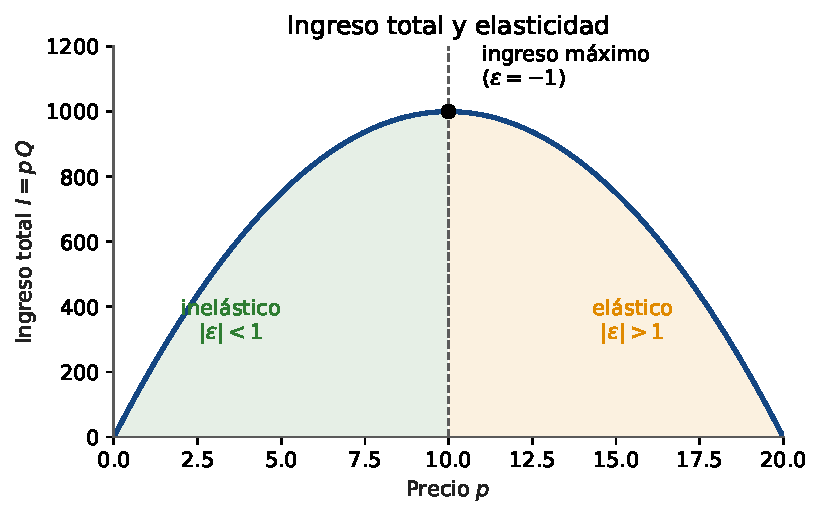
\includegraphics[width=0.72\linewidth]{figuras/elasticidad_ingreso}
\caption{El ingreso total alcanza su máximo cuando la elasticidad es unitaria ($\varepsilon=-1$). En el tramo inelástico conviene subir el precio; en el elástico, bajarlo.}
\label{fig:elasticidad_ingreso}
\end{figure}

\section{Otras elasticidades}

El concepto se extiende a cualquier par de variables:
\begin{itemize}
  \item \textbf{Elasticidad ingreso de la demanda} $\varepsilon_R = \dfrac{\%\,\Delta Q}{\%\,\Delta R}$ (respecto al ingreso $R$ del consumidor): positiva para bienes \emph{normales}, negativa para bienes \emph{inferiores}.
  \item \textbf{Elasticidad cruzada} $\varepsilon_{xy} = \dfrac{\%\,\Delta Q_x}{\%\,\Delta p_y}$: positiva si los bienes son \emph{sustitutos} (sube el precio del té, subo el consumo de café), negativa si son \emph{complementarios} (sube el precio de la nafta, baja el uso del auto).
\end{itemize}

\begin{ideabox}
\textbf{Por qué importa.} La elasticidad es probablemente el concepto micro más usado en la gestión real: define estrategias de precios, el efecto de un impuesto, la conveniencia de una promoción. Y como es adimensional, permite comparar la sensibilidad de productos tan distintos como la sal y los pasajes de avión.
\end{ideabox}

\begin{labbox}
En la práctica, la elasticidad puntual combina una derivada (\texttt{sympy.diff}) con una evaluación en un punto; la elasticidad arco se calcula directo a partir de dos filas de un \texttt{DataFrame} de \texttt{pandas} con datos reales de precios y cantidades. El curso suele pedir estimarla sobre datos observados: ahí la teoría de este capítulo se encuentra con los datos del laboratorio.
\end{labbox}

\section{Síntesis del capítulo}

La elasticidad mide sensibilidad en términos porcentuales, lo que la hace comparable entre mercados. Su relación con el ingreso total es una herramienta directa de decisión de precios. En el próximo capítulo pasamos de la derivada (medir el cambio) a su operación inversa, la integral (acumular el cambio), para medir el bienestar.
